% !TeX spellcheck = en_US
\documentclass[12pt]{article}

\usepackage{times,fullpage,xspace,fancyhdr,url,color}
\usepackage[pdftex]{graphicx}
\usepackage[pdftex,
            colorlinks=true,
            urlcolor=black,
            linkcolor=black,
            citecolor=black,
            bookmarksopen=false,
            bookmarksnumbered=true,
            pdfstartview=FitH]{hyperref}

\pdfcompresslevel=9
\newcommand{\leaguename}{RoboCup Standard Platform League (NAO) }
\hypersetup{
 pdftitle={Pass Masters: Bridging the Leagues},
 pdfauthor={Technical Committee SPL},
}
\usepackage{microtype}
\usepackage[utf8]{inputenc}
\usepackage{amsmath}
\usepackage{xargs}
\usepackage[colorinlistoftodos,prependcaption,textsize=tiny]{todonotes}
\usepackage{siunitx}
\usepackage[capitalize,noabbrev]{cleveref}
\usepackage[official]{eurosym}
\usepackage[useregional]{datetime2}
\usepackage{subcaption}
\usepackage{enumitem}
\usepackage{xcolor}
\DTMlangsetup[en-GB]{ord=raise,monthyearsep={,\space}}

\newcommandx{\unsure}[2][1=]{\todo[linecolor=red,backgroundcolor=red!25,bordercolor=red,#1]{#2}}
\newcommandx{\change}[2][1=]{\todo[linecolor=blue,backgroundcolor=blue!25,bordercolor=blue,#1]{#2}}
\newcommandx{\info}[2][1=]{\todo[linecolor=green,backgroundcolor=green!25,bordercolor=green,#1]{#2}}
\newcommandx{\improvement}[2][1=]{\todo[linecolor=Plum,backgroundcolor=Plum!25,bordercolor=Plum,#1]{#2}}


\usepackage[theorems]{tcolorbox}
\newtcbtheorem[number within=section]{hintbox}{}%
{colback=red!10,colframe=red!45!black,fonttitle=\bfseries}{th}

% !TeX root = ../SPL-Rules.tex
% !TeX spellcheck = en_US
\newcommand{\TotalWidth}{7.4}
\newcommand{\TotalLength}{10.4}
\newcommand{\GoalScoredDelay}{15}
\newcommand{\KickOffAutoTime}{45}
\newcommand{\KickOffBallFreeTime}{10}
\newcommand{\FreeKickTime}{30}
\newcommand{\FreeKickRadius}{0.75}
\newcommand{\VisualSignalTime}{2}
\newcommand{\ReadyDelayTimeChampion}{45}
\newcommand{\ReadyDelayTimeChallenge}{40}
\newcommand{\PlayingDelayTime}{15}
\newcommand{\PenaltyKickTime}{30}
\newcommand{\PenaltyKickSetupTime}{30}
\newcommand{\PenaltyShootoutKickTime}{30}
\newcommand{\StandardPenaltyTime}{45}
\newcommand{\StandardPenaltyIncrease}{10}
\newcommand{\NovelContributionTime}{3 years\xspace}
\newcommand{\GameStuckTime}{30}
\newcommand{\TeamMessageSize}{128}
\newcommand{\TeamMessageLimit}{1200} % Limit of number of packets available to one team during a game with two halves of 10 minutes.
\newcommand{\TeamMessageLimitMinute}{60} % Limit for the average number of packets available to one team during a minute of gameplay.
\newcommand{\MaxJerseyNumber}{20} % the highest allowed jersey number to wear by robot players

% !TeX root = ../SPL-Rules.tex
% !TeX spellcheck = en_US
\newcommand{\LastRCYear}{2022\xspace}
\newcommand{\RCYear}{2023\xspace}
\newcommand{\JerseyApproveSubmissionDate}{2023-05-01}
\newcommand{\CodeReleaseAnnouncementDate}{2023-10-15}


\sloppy
\newcommand{\ie}{\mbox{i.\,e.}\xspace}
\newcommand{\eg}{\mbox{e.\,g.}\xspace}
%\newcommand{\cf}{\mbox{cf.}\xspace}
\newcommand{\cf}{see\xspace}
% \newcommand{\comment}[1]{\marginpar{\pdfannot width 4in height .5in depth 8pt {/Subtype /Text /Contents (#1)}}}
\newcommand{\inparagraph}[1]{\paragraph{#1\hspace{-1em} }}


% some colors
\definecolor{orange}{rgb}{1,0.5,0}
\definecolor{red}{rgb}{1,0,0}
\definecolor{green}{rgb}{0,1,0}


\title{\leaguename\\RoboCup Soccer Humanoid League (HL)
\\Pass Masters: Bridging the Leagues}
\author{RoboCup SPL-HL Technical Committee}
\date{(\RCYear SPL-HL Challenge, as of \today)}

\setlength{\parindent}{0pt}
\setlength{\parskip}{12pt plus 6pt minus 3 pt}
\setcounter{tocdepth}{1}
\widowpenalty=10000
\clubpenalty=10000

\pagestyle{fancy}
\lhead{}
\chead{}
\rhead{}
\lfoot{}
\cfoot{}
\rfoot{}

\renewcommand{\headrulewidth}{0.4pt}
\renewcommand{\footrulewidth}{0.4pt}

% needed to align an image and text correctly side by side
\newcommand{\imagebox}[1]{\raisebox{2ex}{\raisebox{-\height}{#1}}}

\begin{document}

\maketitle
\thispagestyle{empty}

\begin{center}
Questions or comments on the challenge should be submitted via \url{https://github.com/RoboCup-SPL/Rules/issues}, to the \texttt{\#rule-book} channel on the SPL Discord server, or by mail both \url{rc-spl-tc@lists.robocup.org} and \url{rc-hl-tc@lists.robocup.org}.
\end{center}

\newpage


\thispagestyle{fancy}

\clearpage

\cfoot{\thepage}
\setcounter{page}{1}


\section{Idea of the Challenge}
Teamwork is a crucial aspect of soccer, and passing the ball between teammates is a fundamental component of successful collaboration.
This challenge is designed to encourage teams to develop effective offensive passing strategies while fostering cooperation between robots from different leagues.

In each session, teams will collaborate with a different team.
The total number of sessions will be finalized closer to the competition.

The challenge involves two robots from the Standard Platform League (SPL) and two robots from the Humanoid League (HL).
One robot from each league will form a cooperative team, while the other two robots will act as static obstacles.
Each obstacle robot will face the attacking robot from the opposite league. 

The objective for the attacking robots is to complete as many successful passes as possible within a five-minute period.
To promote collaboration, the challenge aims to maximize the number of attempts, enabling teams to cooperate with as many participating teams from the other league as possible.
However, the exact number of attempts will be determined closer to the competition, based on the available schedule and time constraints.
\begin{figure}[ht]
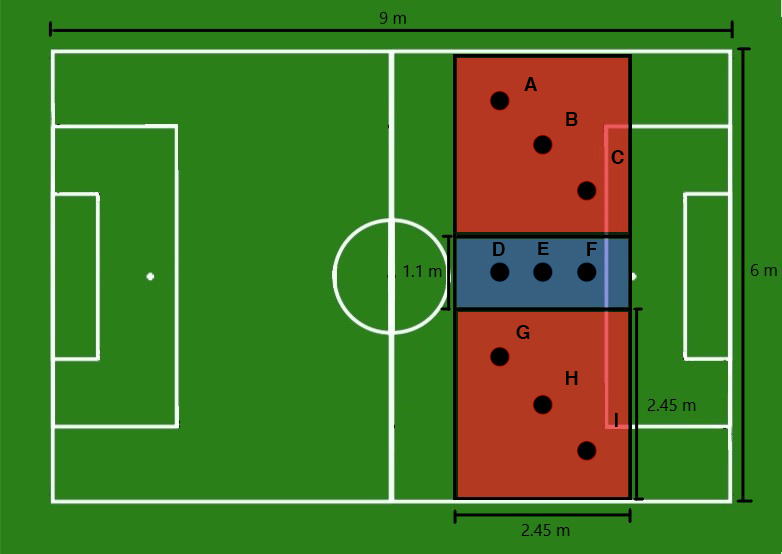
\includegraphics[width=0.95\linewidth]{figs/ch_2_full.jpg}
\caption{Setup using the standard SPL field. The red zones are for attacking robots, and the blue zone for defending robots. }
\label{ch2:zone96}
\centering
\end{figure}

\section{Field Setup}
This challenge will be conducted on a standard SPL field.
The challenge requires three virtual zones shown in Figure \ref{ch2:zone96}.
The red zones represent area available to attacker robots. The blue zone represents the area where the defender robots are placed.
The three zones should be made clearly visible to observers including the referee, by demarcating them on the field through the use of a green tape. The tape must not break the regular white field lines.
Robots must localize using the regular filed lines.
The ball used must be from the Humanoid league, featuring a dark-and-white patterned design.

\section{Network communication}
The two attacking robots must be connected to the GameController.
Direct network-based communication between the robots is prohibited.
However, other forms of natural communication, such as visual signal or sound is allowed.

\section{Robots positioning}
The defending robots must be turned on and stay in a standing position facing the attacking from the other league.
They must remain in the same static position toward the attempt.
The starting robot's positions are identified by the points ${A,B,C,D,E,F,G,H,I}$ in Figures \ref{ch2:zone96}.
The robot's positions are:

\textbf{Standard SPL field} the reference frame of each point is put in the lower left corner of the corresponding area.
\\
$A = G = (0.6m, 1.8m)$
\\
$B = H = (1.2m, 1.2m)$
\\
$C = I = (1.8m, 0.6m)$
\\
$D = (0.6, 0.55m)$
\\
$E = (1.2m, 0.55m)$
\\
$F = (1.8m, 0.55m)$
\\
\\

One attacking robots is randomly placed in A, B, or C, and the other attacking robot randomly at G, H, or I.
One attacking robot is randomly selected to start with the ball.
The defenders are positioned randomly D, E, or F.
See Figure \ref{ch2:zone96}.
In case of fallen robots, if the robot is not able to get up by itself, the team can request a fallen robot from the GameController.
This will obviously result in a penalization for the robot and a possible time loss for the team.

\section{Challenge Execution}
For each attempt the attacking robots must be connected to GameController.
Before each attempt, GameController is set to Initial.
After the robots are positioned, the GameController changes to Ready state and then Set.
The attempt commences using the referee whistle and GameController process, as in typical SPL games.

The attacking robots pass the ball back-and-forth as often as possible until the attempt ends.
The attacking robots must remain within their red zones throughout the attempt.
A robot is considered inside its red zone if any part of the robot remains within the virtual plane of the zone.

If the ball leaves the red zones and comes to a full stop, the cooperative teams get one possibility of resetting the ball.
The ball must be placed approximately 30 cm in front of the last attacking robot that touched the ball.

An attempt ends when:
\begin{enumerate}
    \item The timeout is reached,
    \item The defenders touch the ball,
    \item One attacking player leave its red zone.
\end{enumerate}

Each team may make three attempts at the challenge however, they cannot modify their code between the attempts.

\section{Passing definition}
\label{sec:pass-definition}
A successful pass is defined as meeting all the following criteria:
\begin{enumerate}
    \item The ball has been touched by two attacking robots.
    \item The ball moved more than one meter from its starting position.
    \item The ball crosses the blue zone so that is starts and ends in different red zones.
    \item The ball stops moving in a red zone.
\end{enumerate}

\section{Scoring and Overall Ranking}
One point is awarded for each successful pass (\cf Section~\ref{sec:pass-definition}). The referee will count and adjudicate successful passes.
The score for an attempt is the total number of successful passes.

Teams are ranked overall based on their score, from the highest to the lowest.

\end{document}
